\documentclass[tikz,border=4pt]{standalone}
\usepackage{tikz}
\usetikzlibrary{shapes.geometric,arrows.meta}

\begin{document}
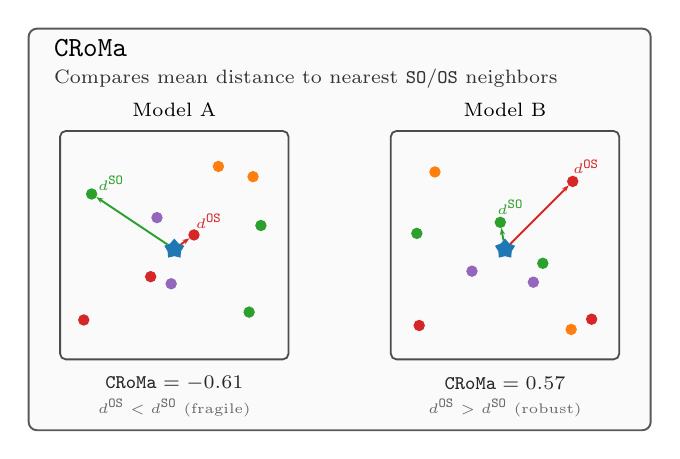
\begin{tikzpicture}[font=\small]
  \definecolor{anchorblue}{RGB}{31,119,180}
  \definecolor{sscol}{RGB}{148,103,189}
  \definecolor{oocol}{RGB}{255,127,14}
  \definecolor{socol}{RGB}{44,160,44}
  \definecolor{oscol}{RGB}{214,39,40}

  \tikzset{
    anchorpt/.style={star,star points=5,fill=anchorblue,draw=anchorblue,minimum size=7pt,inner sep=0pt},
    sspoint/.style={circle,draw=sscol,fill=sscol,minimum size=3.7pt,inner sep=0pt},
    oopoint/.style={circle,draw=oocol,fill=oocol,minimum size=3.7pt,inner sep=0pt},
    sopoint/.style={circle,draw=socol,fill=socol,minimum size=3.7pt,inner sep=0pt},
    ospoint/.style={circle,draw=oscol,fill=oscol,minimum size=3.7pt,inner sep=0pt},
    repspace/.style={draw=black!70,line width=0.65pt},
    distarrow/.style={-{Stealth[length=2.5pt]},line width=0.7pt},
    panelframe/.style={rounded corners=3pt,draw=black!65,fill=black!2,line width=0.7pt}
  }

  \draw[panelframe] (-1.85,-2.55) rectangle (6.05,2.55);
  \node[anchor=west,font=\bfseries] at (-1.65,2.30) {\texttt{CRoMa}};
  \node[anchor=west,font=\scriptsize,text=black!80] at (-1.65,1.92)
    {Compares mean distance to nearest \texttt{SO}/\texttt{OS} neighbors};

  % ---------------- Model A: CRoMa < 0 (fragile) ----------------
  \begin{scope}[shift={(0,-0.25)}]
    \draw[repspace,rounded corners=2pt] (-1.45,-1.40) rectangle (1.45,1.50);
    \node[anchor=south,font=\scriptsize] at (0,1.56) {Model A};

    % Anchor
    \node[anchorpt] (ancA) at (0,0) {};

    % SO neighbors (farther)
    \node[sopoint] (soA1) at (-1.05,0.70) {};
    \node[sopoint] (soA2) at (0.95,-0.80) {};

    % OS neighbors (closer)
    \node[ospoint] (osA1) at (0.25,0.18) {};
    \node[ospoint] (osA2) at (-0.30,-0.35) {};

    % Other scattered points (context)
    \node[sopoint] at (1.10,0.30) {};
    \node[ospoint] at (-1.15,-0.90) {};
    \node[sspoint] at (-0.04,-0.44) {};
    \node[oopoint] at (0.56,1.05) {};
    \node[sspoint] at (-0.22,0.40) {};
    \node[oopoint] at (1.00,0.92) {};

    % Distance arrows to nearest SO
    \draw[distarrow,socol] (ancA) -- (soA1);
    \node[anchor=south east,font=\tiny,text=socol] at (-0.51,0.62) {$d^{\texttt{SO}}$};

    % Distance arrows to nearest OS
    \draw[distarrow,oscol] (ancA) -- (osA1);
    \node[anchor=south west,font=\tiny,text=oscol] at (0.15,0.14) {$d^{\texttt{OS}}$};

    \node[font=\scriptsize,text=black!85] at (0,-1.70) {$\texttt{CRoMa} = -0.61$};
    \node[font=\tiny,text=black!60] at (0,-2.02) {$d^{\texttt{OS}} < d^{\texttt{SO}}$ (fragile)};
  \end{scope}

  % ---------------- Model B: CRoMa > 0 (robust) ----------------
  \begin{scope}[shift={(4.20,-0.25)}]
    \draw[repspace,rounded corners=2pt] (-1.45,-1.40) rectangle (1.45,1.50);
    \node[anchor=south,font=\scriptsize] at (0,1.56) {Model B};

    % Anchor
    \node[anchorpt] (ancB) at (0,0) {};

    % SO neighbors (closer)
    \node[sopoint] (soB1) at (-0.06,0.34) {};
    \node[sopoint] (soB2) at (0.48,-0.18) {};

    % OS neighbors (farther)
    \node[ospoint] (osB1) at (0.86,0.86) {};
    \node[ospoint] (osB2) at (-1.09,-0.97) {};

    % Other scattered points (context)
    \node[sopoint] at (-1.12,0.20) {};
    \node[ospoint] at (1.10,-0.89) {};
    \node[sspoint] at (0.36,-0.42) {};
    \node[oopoint] at (0.84,-1.02) {};
    \node[sspoint] at (-0.42,-0.28) {};
    \node[oopoint] at (-0.89,0.98) {};

    % Distance arrows to nearest SO
    \draw[distarrow,socol] (ancB) -- (soB1);
    \node[anchor=south west,font=\tiny,text=socol] at (-0.22,0.32) {$d^{\texttt{SO}}$};

    % Distance arrows to nearest OS
    \draw[distarrow,oscol] (ancB) -- (osB1);
    \node[anchor=south west,font=\tiny,text=oscol] at (0.74,0.83) {$d^{\texttt{OS}}$};

    \node[font=\scriptsize,text=black!85] at (0,-1.70) {$\texttt{CRoMa} = 0.57$};
    \node[font=\tiny,text=black!60] at (0,-2.02) {$d^{\texttt{OS}} > d^{\texttt{SO}}$ (robust)};
  \end{scope}

  % Legend removed: shared across the Fig 1 composite (see figures/concept_legend.tex).
\end{tikzpicture}
\end{document}
